\underbar{\textbf{\large Ejercicio 1:}} Se dispone de una clase base Persona y dos clases especializadas Alumno y Profesor. Se quiere saber qué alumnos están matriculados en qué asignaturas y qué profesores imparten qué asignaturas, y viceversa. 

Para ello hay dos opciones:
\begin{itemize}
  \item Dos asociaciones bidireccionales varios a varios, una entre Alumno y Asignatura, y otra entre Profesor y Asignatura.
  \item Una única asociación bidireccional varios a varios entre las clases Persona y Asignatura.
\end{itemize}
Como queremos que solamente accedan a las asignaturas ya sean Alumnos o Profesores si lo implementamos mediante la segunda manera cualquier Persona que no sea ni Alumno ni Profesor podrá acceder a las asignatura, como eso es algo que no queremos lo implementaremos mediante la primera manera.

\begin{figure}[h]
  \begin{center}
    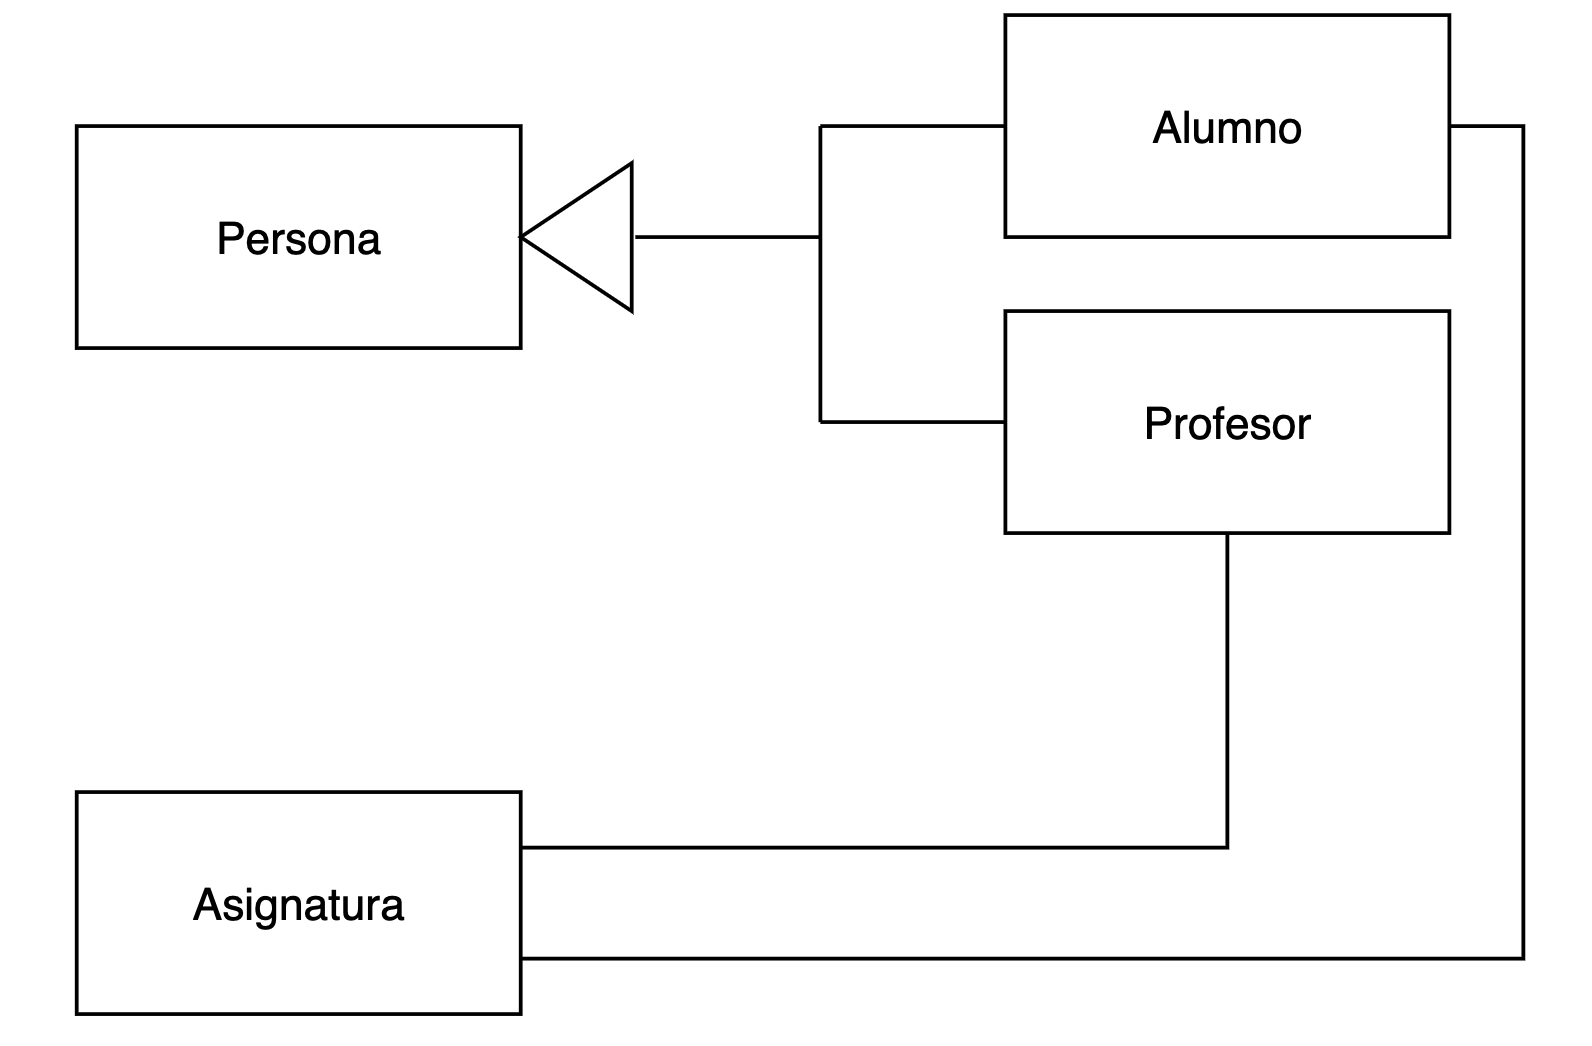
\includegraphics[width=\textwidth]{assets/Seminario3_2_1.png}
  \end{center}
  \caption{Resultado de la implementación del ejercicio}
\end{figure}
\newpage
\underbar{\textbf{\large Ejercicio 2:}} Supóngase que existen ya definidas dos clases Ventana (ventana gráfica), y Barra (barra de desplazamiento) y se quiere definir una nueva clase VentanaBarra (ventana con barra de desplazamiento). Indique si definiría la nueva clase utilizando alguna de las anteriores o como una nueva clase independiente. En caso de utilizar alguna de las ya definidas explique qué relaciones son las que se establecen entre ellas y cómo las codificaría. Razone la respuesta.

Una VentanaBarra estará compuesta por una Ventana y una Barra, por tanto, podriamos implementarla como dos composiciones 1-1:
\begin{minted}[breaklines]{C++}
class Ventana{};
class Barra{};
class VentanaBarra{
  public:
    VentanaBarra(Ventana& v, Barra& b):ventana_(v),barras_(b){}
  private:
    Ventana ventana_;
    Barra barras_;
};
\end{minted}

\underbar{\textbf{\large Ejercicio 3:}} Dadas las clases A y B, indicar qué asignaciones son correctas:
\begin{figure}[h]
\begin{minipage}{0.35\textwidth}
\begin{lstlisting}[frame = single]
class A{};
class B: public A {};
int main() {
  A objA, *pA;
  B objB, *pB;
  pA = &objA;
  pB = &objB;
  objA = objB;
  objA = (A)objB;
  objB = objA;
  objB = (B)objA;
  pA=pB;
  pB=pA;
  pB = (B*)pA;
}
\end{lstlisting}
\end{minipage}
\hfill
\begin{minipage}{0.6\textwidth}
Asignaciones:\\
\texttt{pA = \&objA;}→  \\
\texttt{pB = \&objB;}→  \\
\texttt{bjA = objB;}→  \\
\texttt{objA = (A)objB;}→  \\
\texttt{objB = objA;}→  \\
\texttt{objB = (B)objA;}→  \\
\texttt{pA=pB;}→  \\
\texttt{pB=pA;}→  \\
\texttt{pB = (B*)pA;}→  \\

\end{minipage}
\end{figure}

\underbar{\textbf{\large Ejercicio 4:}}
\underbar{\textbf{\large Ejercicio 5:}}
\underbar{\textbf{\large Ejercicio 6:}}